\documentclass[letterpaper]{article}
\usepackage{amssymb}
\usepackage{fullpage}
\usepackage{changepage}
\usepackage{amsmath}
\usepackage{epsfig,float,alltt}
\usepackage{psfrag,xr}
\usepackage[T1]{fontenc}
\usepackage{url}
\usepackage{pdfpages}
\usepackage{epstopdf}
\usepackage[framed,numbered,autolinebreaks,useliterate]{mcode}

%\includepdfset{pagecommand=\thispagestyle{fancy}}
\author{Yi Yang}
\title{Peer Review}

\begin{document}
\date{12/19/2016}
\maketitle

\newcommand{\trace}{\mathrm{trace}}
\newcommand{\real}{\mathbb R}  % real numbers  {I\!\!R}
\newcommand{\nat}{\mathbb N}   % Natural numbers {I\!\!N}
\newcommand{\cp}{\mathbb C}    % complex numbers  {I\!\!\!\!C}
\newcommand{\ds}{\displaystyle}
\newcommand{\mf}[2]{\frac{\ds #1}{\ds #2}}
\newcommand{\spanof}[1]{\textrm{span} \{ #1 \}}
\newcommand{\sol}[0]{\textbf{Solution: }}
\newcommand{\pf}[0]{\textbf{Proof:}}
\newcommand{\rme}[0]{\textrm{e}}
\newcommand{\Null}[1]{\textrm{Null}\{#1\}}
\parindent 0pt
%%%%%%%%%%%%%%%%%%%%%%%%%%%%%%%%%%%%%%%%%%%%%%%%%%%%%%%%%%%%%%%%%%%%%%%%%%%%%%%
% Solution for Question 1 begins here - by Yi Yang
%%%%%%%%%%%%%%%%%%%%%%%%%%%%%%%%%%%%%%%%%%%%%%%%%%%%%%%%%%%%%%%%%%%%%%%%%%%%%%%
\section{\underline{Assessment of Orange Grading by Computer Vision Techniques}}
\begin{itemize}
	\item Group member: Xinrui Zhang, Pin-Chia Chen, Hung-Wen Chen
	\item Background: Traditional way for quality assessment for fruits like oranges by man power is costly and this project presents an assessment method based on computer vision composed of a supervised machine learning algorithm for classification of typical orange features that will indicate the degrees of quality of oranges. These features include texture, color, shape and scar detection. For texture, color and shape detection and classification methods, as clearified in the report, have been completely formulated and solved by previous researchers. However, for this project, Zhang, Xinrui, Pin-Chia and Hung-Wen applied multi-class SVM method instead of neural network method. Except for that, this group also provide the standards and formulation for scar detection on the surface of orange, this procedure will consider several factors such as light reflection, noise, etc.
	\item Technical Description: This project follows the following steps: 1. collecting orange data and label the oranges according to the United States Department of Agriculture (USDA) orange classification standard to generate object images and label sets; 2. preprocessing images to obtain denoised and standard-size orange images; 3. extracting three different features of orange from the normalized images to construct dataset including training set and testing set, which are color, shape, and texture containing several parameters contributing to he grading process; 4. training dataset to build multi-class classification. This procedure can be described by the following scheme.
	\begin{figure}[H]
	\centering
	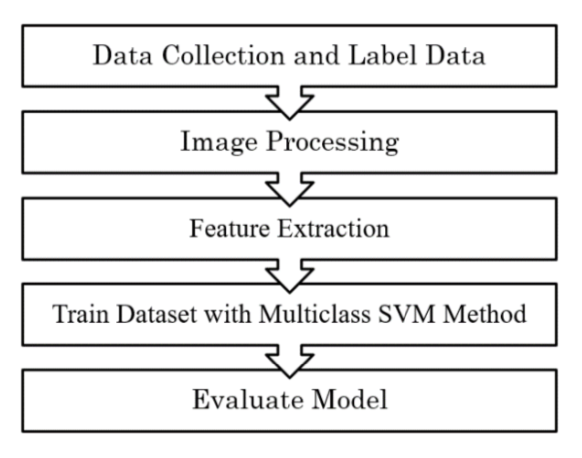
\includegraphics[scale=0.3]{scheme.png}
	\caption{Technical description}
	\label{tech}
	\end{figure}
	
	\item Experimental Results and Analysis: There are in total of 133 images to serve as dataset with 67 sets used as training data and 66 sets used as testing data and plotted the curve of accuracy based on different feature extraction with or without elimination of blare. In this paper, each feature serves to represent different characteristic of each orange. Through experimental results, it can be analyzed whether each feature effectively influence the accuracy of classifying oranges into three different classes with ECOC model. It is observed that accuracy increases as all three feature are weighted in ECOC model.\\
	
	In this report, the feasibility of using computer vision techniques and error-correcting output code multiclass modle to classify the quality naval orange was investigated. It was concluded that the grading accuracy was more robust by reflection elimination and defect detection. Visual resluts also showed that it was necessary to extract more features, normalize extracted features and build a model like ECOC model to build a more accurate, non-destructive, and cost-efficient orange quality evaluation system. 
	\item Suggestions: I think this is an excellent project report in overall. The author illustrated the basic principles and theory of computer vision techniques and presented the details of technical considerations for system modelling. However, several tiny parts I think still need to be considered: 1. If we chose to use detect the scar based on intensity of RGB, we need to consider the effects of previous blurring procedure, which is aimed to eliminate the noise and light reflection. 2. Figures that shows experimental results are not clear enough, you should enlarge the scale the figures presented in your report.
\end{itemize}

\clearpage

\section{\underline{Distracted Driver Detection}}
\begin{itemize}
	\item Group member: Venkatesh Sriram, Chandana Neerukonda and Sabarish Balakrishnan
	\item Background: The United States Department of Transportations motor vehicle safety division has reported that one in five car accidents is caused by a distracted driver. This translates to approximately 425000 injuries and 3000 fatalities caused by distracted driving every year in the United States. This project is inspired by this phenomena to decrease the effects of driver distraction to vehicle crashes that happens every day. This project can be extended to be applied in semi-autonomous vehicle industry for driver behaviour modelling. Based on my own experience, if we can predict the drivers' behaviour based on computer vision techniques, it can be combined with model predictive control scheme applied to vehicle navigation.
	\item Technical Description: The data set contains aound 22000 images taken in the same direction. All are 2D Dashboard image frames. The entire database of 22424 images was split into training set and test set without any overlapping images between them. The images in the data set are divided into 10 categories. The objective is to classify the images into the above ten categories. Handcrafted features and Deep Learning methods are used respectively to classify the data set. The procedure for handcrafted features is shown in figure \ref{hand} and scheme for deep learing or CNN is explained in detailed in report.
	\begin{figure}[H]
	\centering
	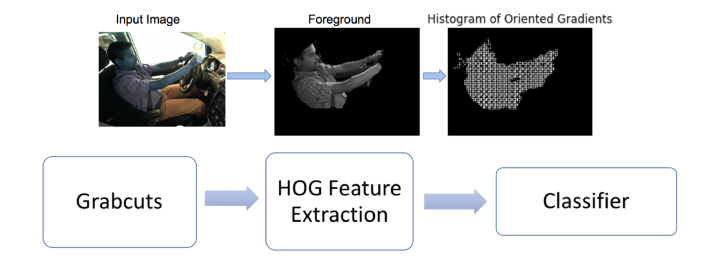
\includegraphics[scale=0.5]{hand.png}
	\caption{Handcrafted features method pipeline}
	\label{hand}
	\end{figure}
	
	\item Experimental Results: From experiments, it can be observed that SVM classifier with Linear kernels gives highest accuracy so far. the confusion matrix of he predicted labels against the true labels. For deep learning algorithm, the tranined AlexNet model over 1000 iterations resulted in a test accuracy of 97.8$\%$. Besides that, the high correlation as an indication of uniform accuracy across all the ten different classes can be observed. It is observed that the method of using HOG features from Grabcuts has given a decent test accuracy of 92.54$\%$. The deep learning based approach showed an accuracy of 97.8$\%$ showing a significant boost over the handcrafted features method. It can be concluded that deep learing method hold more potential in classification tasks of images. A good overvation is that the concept of transfer learning helps in achieving models in faster time and smaller data sizes as well. There are multiple approaches through which more accurate models using deep learning methods can be acquired. As we discussed data size is a prominent thing for training and the knowledge of trained model depends on it. 
	\item Suggestions: Generally speaking, this is an excellent project report. The group members have done series of investigation and literature reviews, this is highly demanding project and if possible could be fully extended to industrial applications. The main issues involve: 1. ten different kinds of human behaviour can not enumerate all the distraction behaviour that human can display; 2. The data set is so large and the speed for computation is a little slow, it is hard to detect the behaviour of driver in real time and I suspect that the frequency of human motions will also affect the accuracy of this two schemes. In overall, computer vision techniques applied to drivers' distraction behaviour detection is a hard work and deserves more real experiments and tests for model calibration.
\end{itemize}

\end{document}